


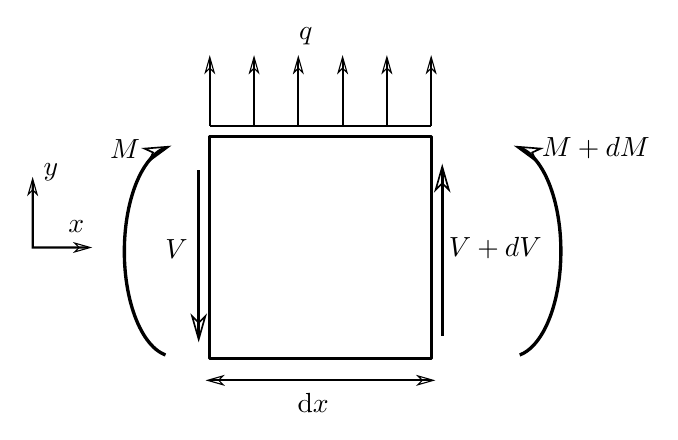
\begin{tikzpicture}[y=0.80pt, x=0.8pt,yscale=-1, inner sep=0pt, outer sep=0pt]
\begin{scope}[shift={(0,-752.36218)}]
  \path[draw=black,fill=black,line join=round,miter limit=4.00,fill
    opacity=0.000,nonzero rule,line width=1.200pt,rounded corners=0.0000cm]
    (95.0000,852.3622) rectangle (195.0000,952.3622);
    \path[color=black,fill=black,line width=0.800pt] (95.0000,961.8750) --
      (95.0000,962.8750) -- (195.0000,962.8750) -- (195.0000,961.8750) --
      (95.0000,961.8750) -- cycle;
    \path[draw=black,even odd rule,line width=0.400pt] (99.0000,962.3622) --
      (101.0000,960.3622) -- (94.0000,962.3622) -- (101.0000,964.3622) --
      (99.0000,962.3622) -- cycle;
    \path[draw=black,even odd rule,line width=0.400pt] (191.0000,962.3622) --
      (189.0000,964.3622) -- (196.0000,962.3622) -- (189.0000,960.3622) --
      (191.0000,962.3622) -- cycle;
    \path[color=black,fill=black,line width=1.200pt] (199.2500,867.3750) --
      (199.2500,942.3750) -- (200.7500,942.3750) -- (200.7500,867.3750) --
      (199.2500,867.3750) -- cycle;
    \path[draw=black,even odd rule,line width=0.600pt] (200.0000,873.3622) --
      (203.0000,876.3622) -- (200.0000,865.8622) -- (197.0000,876.3622) --
      (200.0000,873.3622) -- cycle;
    \path[color=black,fill=black,line width=1.200pt] (89.2500,867.3750) --
      (89.2500,942.3750) -- (90.7500,942.3750) -- (90.7500,867.3750) --
      (89.2500,867.3750) -- cycle;
    \path[draw=black,even odd rule,line width=0.600pt] (90.0000,936.3622) --
      (87.0000,933.3622) -- (90.0000,943.8622) -- (93.0000,933.3622) --
      (90.0000,936.3622) -- cycle;
    \path[color=black,fill=black,nonzero rule,line width=1.200pt] (74.7508,856.6718)
      .. controls (69.8130,858.5099) and (65.5561,863.3884) .. (62.3133,870.2343) ..
      controls (59.0705,877.0802) and (56.8284,885.9197) .. (56.0008,895.8280) ..
      controls (54.9137,908.8435) and (56.4098,921.5363) .. (59.7508,931.6093) ..
      controls (63.0918,941.6823) and (68.2689,949.1964) .. (74.7508,951.6093) --
      (75.2508,950.2030) .. controls (69.4951,948.0605) and (64.4529,940.9833) ..
      (61.1883,931.1405) .. controls (57.9237,921.2978) and (56.4301,908.7726) ..
      (57.5008,895.9530) .. controls (58.3158,886.1958) and (60.5450,877.4952) ..
      (63.6883,870.8593) .. controls (66.8316,864.2234) and (70.8734,859.7075) ..
      (75.2508,858.0780) -- (74.7508,856.6718) -- cycle;
    \path[draw=black,even odd rule,line width=0.600pt] (69.3769,859.4553) --
      (67.6120,863.3134) -- (76.4058,856.8389) -- (65.5188,857.6904) --
      (69.3769,859.4553) -- cycle;
    \path[color=black,fill=black,nonzero rule,line width=1.200pt]
      (235.2492,856.6718) -- (234.7492,858.0780) .. controls (240.5049,860.2206) and
      (245.5471,867.2978) .. (248.8117,877.1405) .. controls (252.0763,886.9833) and
      (253.5699,899.5085) .. (252.4992,912.3280) .. controls (251.6842,922.0852) and
      (249.4550,930.7859) .. (246.3117,937.4218) .. controls (243.1684,944.0577) and
      (239.1266,948.5735) .. (234.7492,950.2030) -- (235.2492,951.6093) .. controls
      (240.1869,949.7712) and (244.4439,944.8927) .. (247.6867,938.0468) .. controls
      (250.9295,931.2009) and (253.1716,922.3614) .. (253.9992,912.4530) .. controls
      (255.0863,899.4376) and (253.5902,886.7448) .. (250.2492,876.6718) .. controls
      (246.9082,866.5988) and (241.7311,859.0847) .. (235.2492,856.6718) -- cycle;
    \path[draw=black,even odd rule,line width=0.600pt] (240.6231,859.4553) --
      (244.4812,857.6904) -- (233.5942,856.8389) -- (242.3880,863.3134) --
      (240.6231,859.4553) -- cycle;
  \path[fill=black] (134.65359,976.70172) node[above right] (text7264) {d$x$};
  \path[fill=black] (75,907.36218) node[above right] (text7268) {$V$};
  \path[fill=black] (50,862.36218) node[above right] (text7272) {$M$};
  \path[fill=black] (203,907.36218) node[above right] (text7276) {$V+\text{d}V$};
  \path[fill=black] (245,862.36218) node[above right] (text7280) {$M+\text{d}M$};
  \path[draw=black,line join=miter,line cap=butt,line width=0.800pt]
    (95.0000,847.3622) -- (195.0000,847.3622);
    \path[color=black,fill=black,line width=0.800pt] (94.5000,817.3750) --
      (94.5000,847.3750) -- (95.5000,847.3750) -- (95.5000,817.3750) --
      (94.5000,817.3750) -- cycle;
    \path[draw=black,even odd rule,line width=0.400pt] (95.0000,821.3622) --
      (97.0000,823.3622) -- (95.0000,816.3622) -- (93.0000,823.3622) --
      (95.0000,821.3622) -- cycle;
    \path[color=black,fill=black,line width=0.800pt] (174.5000,817.3750) --
      (174.5000,847.3750) -- (175.5000,847.3750) -- (175.5000,817.3750) --
      (174.5000,817.3750) -- cycle;
    \path[draw=black,even odd rule,line width=0.400pt] (175.0000,821.3622) --
      (177.0000,823.3622) -- (175.0000,816.3622) -- (173.0000,823.3622) --
      (175.0000,821.3622) -- cycle;
    \path[color=black,fill=black,line width=0.800pt] (114.5000,817.3750) --
      (114.5000,847.3750) -- (115.5000,847.3750) -- (115.5000,817.3750) --
      (114.5000,817.3750) -- cycle;
    \path[draw=black,even odd rule,line width=0.400pt] (115.0000,821.3622) --
      (117.0000,823.3622) -- (115.0000,816.3622) -- (113.0000,823.3622) --
      (115.0000,821.3622) -- cycle;
    \path[color=black,fill=black,line width=0.800pt] (134.5000,817.3750) --
      (134.5000,847.3750) -- (135.5000,847.3750) -- (135.5000,817.3750) --
      (134.5000,817.3750) -- cycle;
    \path[draw=black,even odd rule,line width=0.400pt] (135.0000,821.3622) --
      (137.0000,823.3622) -- (135.0000,816.3622) -- (133.0000,823.3622) --
      (135.0000,821.3622) -- cycle;
    \path[color=black,fill=black,line width=0.800pt] (194.5000,817.3750) --
      (194.5000,847.3750) -- (195.5000,847.3750) -- (195.5000,817.3750) --
      (194.5000,817.3750) -- cycle;
    \path[draw=black,even odd rule,line width=0.400pt] (195.0000,821.3622) --
      (197.0000,823.3622) -- (195.0000,816.3622) -- (193.0000,823.3622) --
      (195.0000,821.3622) -- cycle;
    \path[color=black,fill=black,line width=0.800pt] (154.5000,817.3750) --
      (154.5000,847.3750) -- (155.5000,847.3750) -- (155.5000,817.3750) --
      (154.5000,817.3750) -- cycle;
    \path[draw=black,even odd rule,line width=0.400pt] (155.0000,821.3622) --
      (157.0000,823.3622) -- (155.0000,816.3622) -- (153.0000,823.3622) --
      (155.0000,821.3622) -- cycle;
  \path[fill=black] (135.3607,810.88519) node[above right] (text7684) {$q$};
    \path[color=black,fill=black,line width=0.800pt] (14.5000,872.3622) --
      (14.5000,902.3622) -- (14.5000,902.8622) -- (15.0000,902.8622) --
      (40.0000,902.8622) -- (40.0000,901.8622) -- (15.5000,901.8622) --
      (15.5000,872.3622) -- (14.5000,872.3622) -- cycle;
    \path[draw=black,even odd rule,line width=0.400pt] (36.0000,902.3622) --
      (34.0000,904.3622) -- (41.0000,902.3622) -- (34.0000,900.3622) --
      (36.0000,902.3622) -- cycle;
    \path[draw=black,even odd rule,line width=0.400pt] (15.0000,876.3622) --
      (17.0000,878.3622) -- (15.0000,871.3622) -- (13.0000,878.3622) --
      (15.0000,876.3622) -- cycle;
  \path[shift={(0,752.36218)},fill=black] (31.112698,143.02229) node[above right]
    (text9186) {$x$};
  \path[fill=black] (20,872.36218) node[above right] (text9190) {$y$};
\end{scope}

\end{tikzpicture}

